
\chapter{Cost, engineering and schedule impact}
\label{cha:engineering}
\section{Outer HCal}
\subsection{Thinned Outer HCal}
\label{ohcal_thin}

\textbf{Cost delta: -\$0.4M}

We investigated reducing the thickness of the outer HCal by 20~cm, or
approxiately one nuclear interaction length.  The thickness of the
outer HCal in the pCDR design is 86.5~cm.  Several possible effects
were investigated through full \geant simulations of the calorimeter
response.  It should be noted that the calorimeter simulations have
recently been compared to data from the FNAL test beam and have been
found to reproduce the measured response quite well.  We looked at the
effect of thinning on the jet energy response, high-$z$ fragmentation
functions.

From a physics perspective, the effect of thinning the outer HCal by
this amount seems to be moderate, and considered by itself, a thinner
outer HCal would still enable the core elements of the sphenix physics
program to be carried out.

From the perspective of the project, the effect of this modification
would be extremely significant.  The outer HCal is the structural
backbone of the sPHENIX structure.  Reducing the radial thickness
significantly reduces the ability of the outer HCal to support the
detector.  The finite element analysis would need to be redone, and
the tilt angle of the steel plates reanalyzed and likely changed. The
prototyping and test beam would have to be redone, delaying plans to
build a full scale mechanical prototype.  The inner HCal will need
some redesign due to the changes in the EMCal, as the $\phi$
segmentation of the two calorimeters should match for mechanical
reasons.  This option sets the outer HCal engineering back as much as
twelve months and requires R\&D be redone.

In the nominal design, the $5.5 \lambda$ total depth of the
calorimeter stack (at $\eta = 0$) is distributed as $1 \lambda$
(EMCal), $1 \lambda$ (inner HCal), and $3.5 \lambda$.  If the outer
HCal is reduced to $2.5 \lambda$, one has to consider the effects if
one or more of the other calorimeters in the stack is also modified.
If the inner HCal is not installed, the depth of the calorimeter stack
is reduced by an additional $1 \lambda$ over the whole acceptance,
falling to $2.5 \lambda$ at midrapidity.  If the EMCal acceptance is
cut to $|\eta| < 0.7$, the thickness of the calorimeter stack in the
range $0.7 < \eta < 1.1$ becomes thinner by $1 \lambda$, but the
effect in that range (aside from the lack of EMCal coverage) is
moderated by the increasing thickness of the calorimeters along lines
of constant $\eta$ due to their rectangular profile.



\chapter*{Shortened HCal}
\label{ohcal_short}

\section*{Inner HCal}
\label{ihcal}

We have considered not building and installing the inner HCal.  One
positive aspect is that by not building a detector, one saves the full
set of costs associated with engineering, prototyping and producing
the detector, not just a fraction of the production costs as would be
saved by building a fraction of the final detector.  The lack of an
active absorber between the outer radius of the EMCal and the cryostat
has pronounced effect on the science capabilities of sPHENIX. The jet
energy response is worsened by removing a full interaction length of
absorber, an effect that is amplified compared to naive expectation
because the volume normally occupied by the inner HCal is in a
1.5~tesla magnetic field.  The lower momentum components of showers
that initiate in the EMCal can be strongly bent in the absorber-free
space before the cryostat.  These particles can also curl around and
strike additional EMCal towers.  Because of these effects, the
colaboration strongly disfavors removing the inner HCal.

From a project perspective, the inner HCal is one of the subsystems
that has the potential to involve non-BNL machine shops.  In
particular, the shop capabilities of some collaborating sPHENIX
Universities could allow them to take a significant role in the
machining and construction of inner HCal modules.  Deciding not to
build this detector would reinforce a view that sPHENIX is essentially
a BNL-only project.

\section{EMCal}

The EMCal accounts for a significant portion of the M\&S budget.  It
also enables the key $\Upsilon$ and direct $\gamma$ and $\gamma+$jet
capabilities of sPHENIX.  

\subsection{Reduction in EMCal Segmentation}
\label{emcal_ganging}
\label{emcal_segmentation}

\textbf{Cost delta: -\$1.7M}

We have considered two options to reduce the electronics cost
associated with the EMCal by reducing the segmentation.  One is
ganging together groups of 2x2 towers in the reference configuration
tower size ($\Delta\eta\times\Delta\phi = 0.024\times0.024$, leading
to an effective segmentation of $0.048 \times 0.048$) and the other is
to make a permanent reduction in the EMCal granularity by making the
towers bigger (one such configuration could be $0.033 \times 0.028$ in
$\Delta \phi x \Delta \eta$), reducing the number of towers by about
38\%. Both options for reducing the segmentation are estimated to
yield approximately the same cost savings.

Ganging together towers means that the R\&D done to date --- both on
production aspects as well as performance in the test beam --- remains
valid.  It does introduce a ``mortgage'' in which the collaboration
would try to identify funds to buy the additional electronics needed
to allow towers be read out individually.

Reducing the EMCal granularity via larger towers would reduce the cost
of the readout electronics, but would likely require increasing the
number of SiPMs per tower to preserve the light collection
uniformity. An advantage of the second option is that this would
provide a finer segmentation than the ganging option, however it would
not allow the reference configuration segmentation to be recovered.
Because this reduced granularity would be a permanent change, it does
not result in a mortgage.

The EMCal R\&D to this point has focused on the production of towers
of the $0.024\times 0.024$ size in the reference configuration.
Increasing the tower size introduces potential production issues in
the tower construction and performance. Additional R\&D will need to
be done to determine if larger towers can be made as efficiently and
uniformly as in the reference configuration and that the light can be
collected from larger area lowers with sufficient uniformity.  If this
option is pursued we would need to pursue R\&D on the larger size
towers to address the concerns described above and based on those
finding to decide which option provides the most feasible construction
option.  This R\&D would delay the overall EMCal schedule by
approximately six months and might require additional prototyping
beyond that which is currently in the schedule.

\subsection{EMCal Coarsened Segmentation}
\label{emcal_segmentation}

\textbf{Cost delta: $-\$1.8M$}

We have investigated reducing the number EMCal towers from
$256\times96=24576$ ($\Delta\eta\times\Delta\phi = 0.024 \times 0.024$) to
$192\times80 = 15360$ ($\Delta\eta\times\Delta\phi = 0.033 \times 0.028$) a
reduction of tower numbers by 37.5\%.  
\chapter*{TPC}
\label{tpc}

\section{MAPS}
\label{maps}

\section{DAQ/Trigger}
\label{daq}

\textbf{Cost delta: -\$1.5M}

The costs associated with the DAQ and Trigger are an area where
significant reductions are achievable.  Although we think the
\$0.5M trigger detector is a suitable target for a non-DOE, possibly
non-US, contribution, for the purposes of answering this charge, we do
not assume that that will happen.  Each of the RHIC experiments has
built trigger detectors that would suit the needs of sPHENIX, and some
of these detectors, such as the trigger detector used by PHOBOS, are
currently unused and available.  We would repurpose one of these
detectors for use in sPHENIX and reduce the M\&S costs accordingly.

We would reuse the infrastructure currently in place in the PHENIX
counting house, consisting of data collection modules (DCMIIs),
subevent buffers (SEBs), assembly and trigger processors (ATPs), a
high throughput networking switch and several racks of computers.
Some amount of new equipment would be needed, such as new level-1 and
global trigger boards.  There is some risk associated with this
approach, as it means, absent funds to renew th computing
infrastructure, starting a new experiment with computing that will be
by then several years old.





\chapter{Physics performance impact}
\label{cha:performance}

Below we describe the simulation studies performed to evaluate the impact of the re-scoping options we identified on the three 
science drivers. We  first compare each change individually to the performance of the reference configuration, and then study
a select set of changes in combination to evaluate their combined effect on the physics performance. For each option we 
describe the simulations employed, ranging from generator level evaluations of count rates to single particle and single jet
\geant simulations + reconstruction to full HIJING central Au+Au \geant simulations and reconstruction. All studies were 
performed for 200 GeV Au+Au collisions.
\section{Hadronic calorimeter changes}
\subsection{Outer HCAL thinning}
The main impact on the science program from thinning the outer HCAL is expected in areas:
\begin{itemize} 
\item Reduced jet energy containment leading the larger systematic uncertainties in the jet energy scale and larger fluctuations
in the jet-by-jet energy measurement.
\item Increased punch-through of high momentum particles leading to a fragmentation function bias
\end{itemize}
The impact was studied with full \geant simulations and jet reconstruction using the \antikt algorithm for single jets 
for the reference configuration, the 20cm thinner oHCAL and the minimal outer HCAL. 
\subsection{Outer HCAL shortening}

For the shortened outer HCAL (reducing the pseudorapidity coverage from $\| \eta \| <$ FIXME to $\| \eta \| < $ FIXME), all measured
at the outer corner of the calorimeter) the expected impact 
is in the statistics of jet related probes. The 20\% reduction in coverage will predominantly affect lower \pt jets ($\pt <$ FIXME),
as jets at the highest \pT have a narrow rapidity distribution that falls within the remaining acceptance. From generator level 
studies, we expect the following loss of statistics: FIXME

Some of the physics impact can be recovered using tracker + EMCal reconstruction of jets, although reduced control over the jet 
energy scale and increased jet-by-jet fluctuations will limit the precision that can be achieved with such studies.

\subsection{Removal of the inner HCAL}

The impact on jet energy scale and fluctuations for this option is expected to be larger than for the outer HCAL thinning, 
with major impact on engineering of the inner detector mechanical design leading to expectations of minimal overall savings.
We therefore did not perform detailed studies of this option.

\section{EMCal}
\subsection{2$\times$2 ganging of EMCal channels}
The reduced EMCal segmentation from 2x2 ganging of readout channels is expected to affect three physics areas: jet finding 
and jet energy reconstruction, electron/hadron separation for the $\Upsilon$ to $e^+ e^-$ channel and photon identification.
We performed full \geant and reconstruction studies of the effect on the single jet response and full \geant simulations for 
Au+Au HIJING events for electron identification. Studies of the effect on photon identification are ongoing.

\subsection{Changing EMCal segmentation}
The reduced EMCal segmentation from increasing the tower dimensions
from $d\eta \times d\phi = 0.024 \times 0.024$ to $0.033 \times 0.28$
was not evaluated with full \geant simulations, as time did not permit
implementing the corresponding detector geometry. However, as the
change increases the tower area by 60\%, as compared to a factor of 4
for the 2x2 ganging, the expected impact can be well estimated based
on the 2x2 ganging full simulations. For the jet response, the 2x2
ganging did not show any noticable effect, implying that the 60\%
increased tower size will also have no effect on jets. For $e/h$
separation, the effect of the 2x2 ganging of about a factor of two
suggests scaling with the $\sqrt{\mbox{area}}$, i.e., the fluctuations
in the background energy. This implies a 26\% change in $e/p$
separation in central Au+Au collisions for the 60\% increase in tower
size, which is well within the projected safety margin for the
measurement.

\subsection{Reduced EMCal pseudorapidity coverage}
Reducing the EMCal coverage will directly affect the expected statistics for $\Upsilon$ to $e^+ e^-$ and photon-based measurements. The 
corresponding loss in statistics is summarized in the table below, based on generator level studies. For jet measurements, the reduced 
coverage leads to a change in jet response across the EMCal boundary. This effect was evaluated by full \geant simulations and reconstruction
of the single jet response in different regions of pseudorapidity and jet \pt.

\section{Outer tracker}

For the outer tracker, the performance of a TPC tracker was evaluated using \geant simulations of single particles, single $\Upsilon$ to $e^+ e^-$
decays, and full HIJING and \geant simulations in a limited acceptance around mid-rapidity (due to timing limitations). Simulations were performed
for an ideal TPC and two configurations with inner field cage boundary at $r=20$~cm and $r=30$~cm. For the latter configurations, effects of 
residual space charge distortions expected after corrections were included. We evaluated general performance characteristics (efficency, fake track
rate, DCA and momentum resolution) and specifically the $\Upsilon$ mass resolutions for the different cases. The TPC simulations were performed
in combination with the 3-layer MAPS configuration of the reference design, and include the effects of track reconstruction and kinematic fits. 
The effect of various inner tracker options on the tracking performance is evaluated separately in \ref{sec:innertracker}.
\subsection{Tracking performance evaluation}

\begin{figure}[hbt]
  \centering
  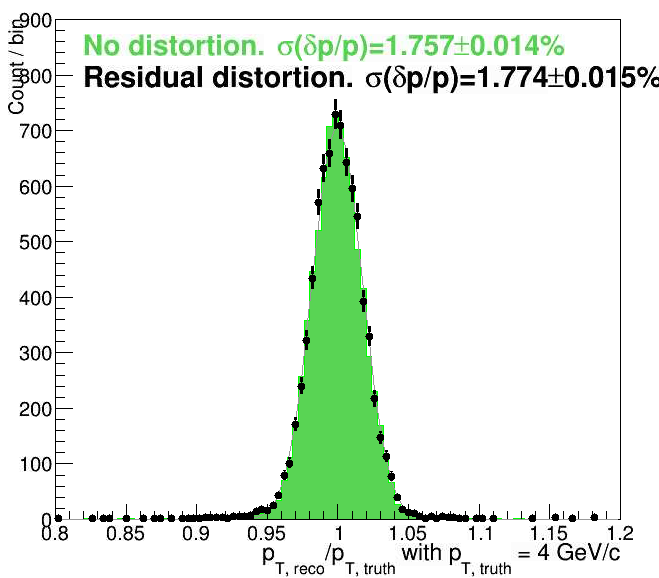
\includegraphics[width=0.4\linewidth]{figs/tpc_residual_correction_20cm}
  \hspace{0.1\linewidth}
  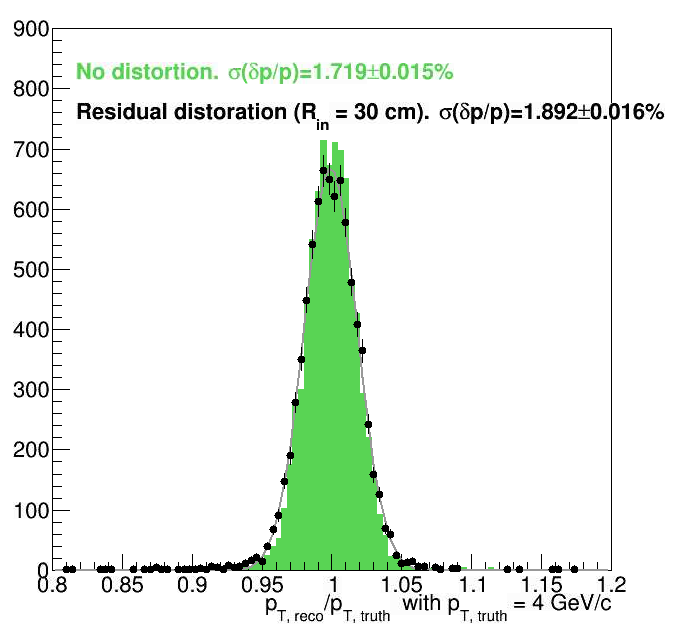
\includegraphics[width=0.4\linewidth]{figs/tpc_residual_correction_30cm}
  \caption{Comparison of residual TPC distortions, after applying
    corrections, for the inner radius at (left) 20~cm and (right)
    30~cm. Leaving 10~cm clear between the inner surface of the field
    cage and the beginning of the tracking volume results in
    significantly smaller residual distortions after correction.}
  \label{fig:tpc_residuals}
\end{figure}

\subsection{$\Upsilon$ mass resolution}


\begin{table}
  \centering
  \begin{tabular}{lr}
    \toprule
    Configuration & $\Upsilon$ mass resolution \\
    \midrule
3 maps layers and 60 TPC layers with no distortion due to space charge
&  66 MeV/$c^2$ \\
3 maps layers and 30 TPC layers with no distortion due to space charge
& 76 MeV/$c^2$ \\
3 maps layers and 60 TPC layers with distortions due to space charge
& 67.4 MeV/$c^2$ \\
3 maps layers and 30 TPC layers with distortions due to space charge
& 77.2 MeV/$c^2$ \\
    \bottomrule
  \end{tabular}
  \caption{Effects of corrected TPC space charge distortions and sparsified readout on the $\Upsilon$ mass resolution.}
  \label{tab:upsilon_mass_resolution}
\end{table}



\section{Inner tracker}
\label{sec:innertracker}
\subsection{VTX pixel configuration}
\subsection{2-layer MAPS tracker}
\section{DAQ and trigger}
\subsection{Minimum bias trigger counter and vertex locator}
\subsection{Offline event building}


\begin{figure}[hbt]
  \centering
  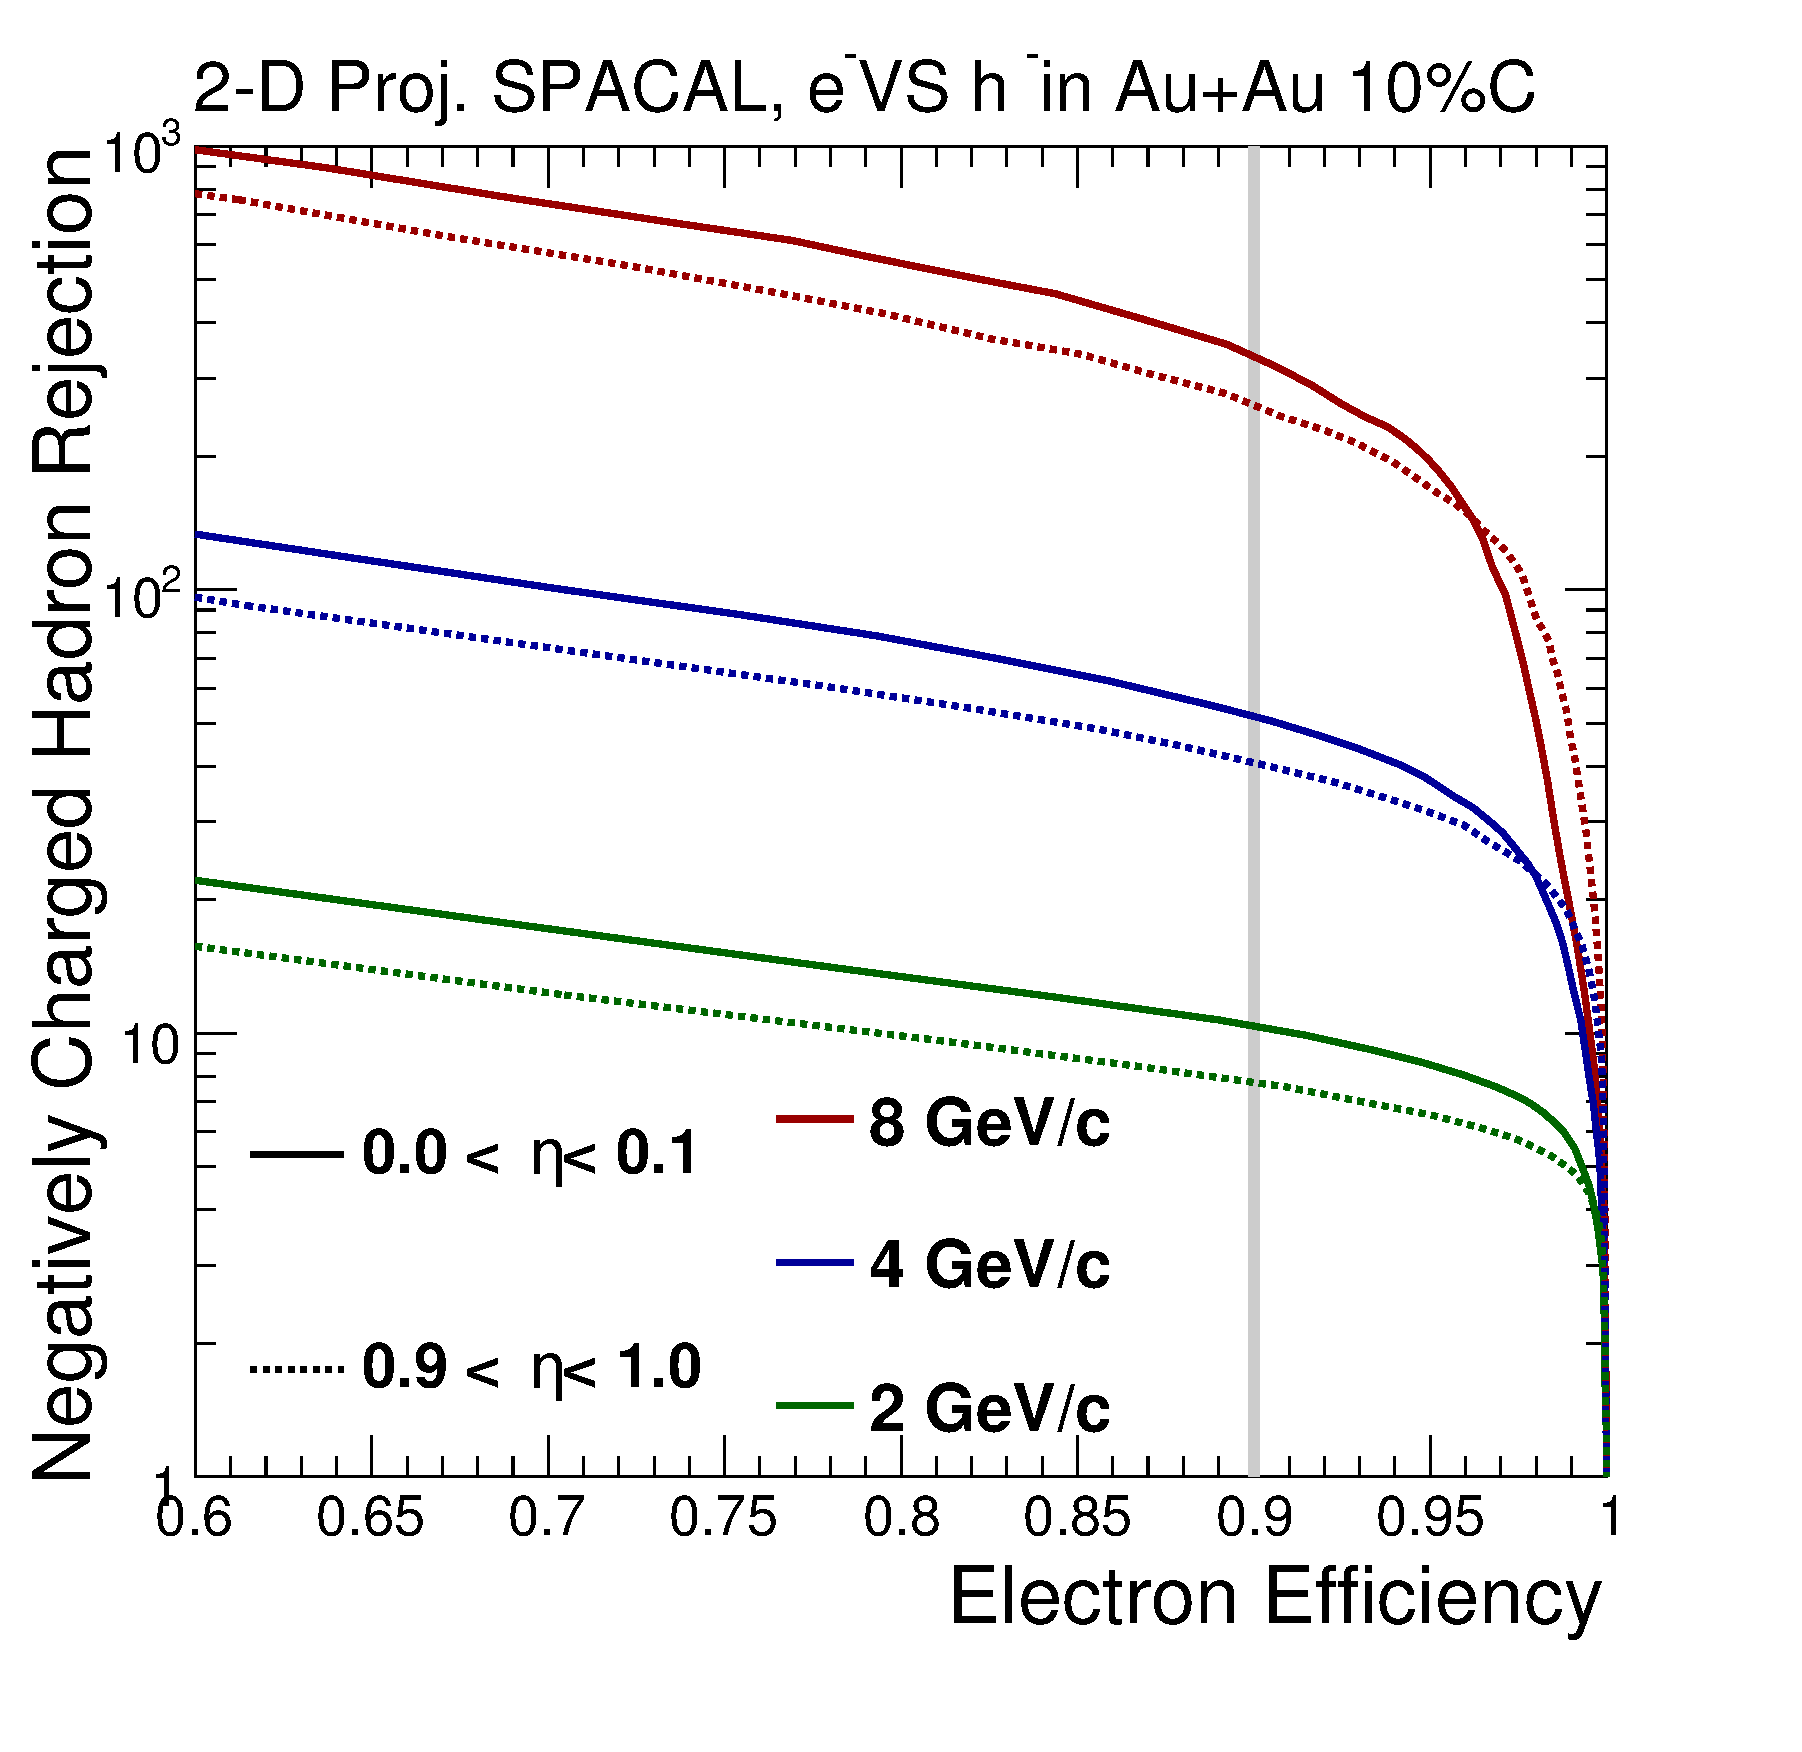
\includegraphics[width=0.4\linewidth]{figs/DrawEcal_Likelihood_Sum_RejectionCurve_AuAuSummary}
  \hspace{0.1\linewidth}
  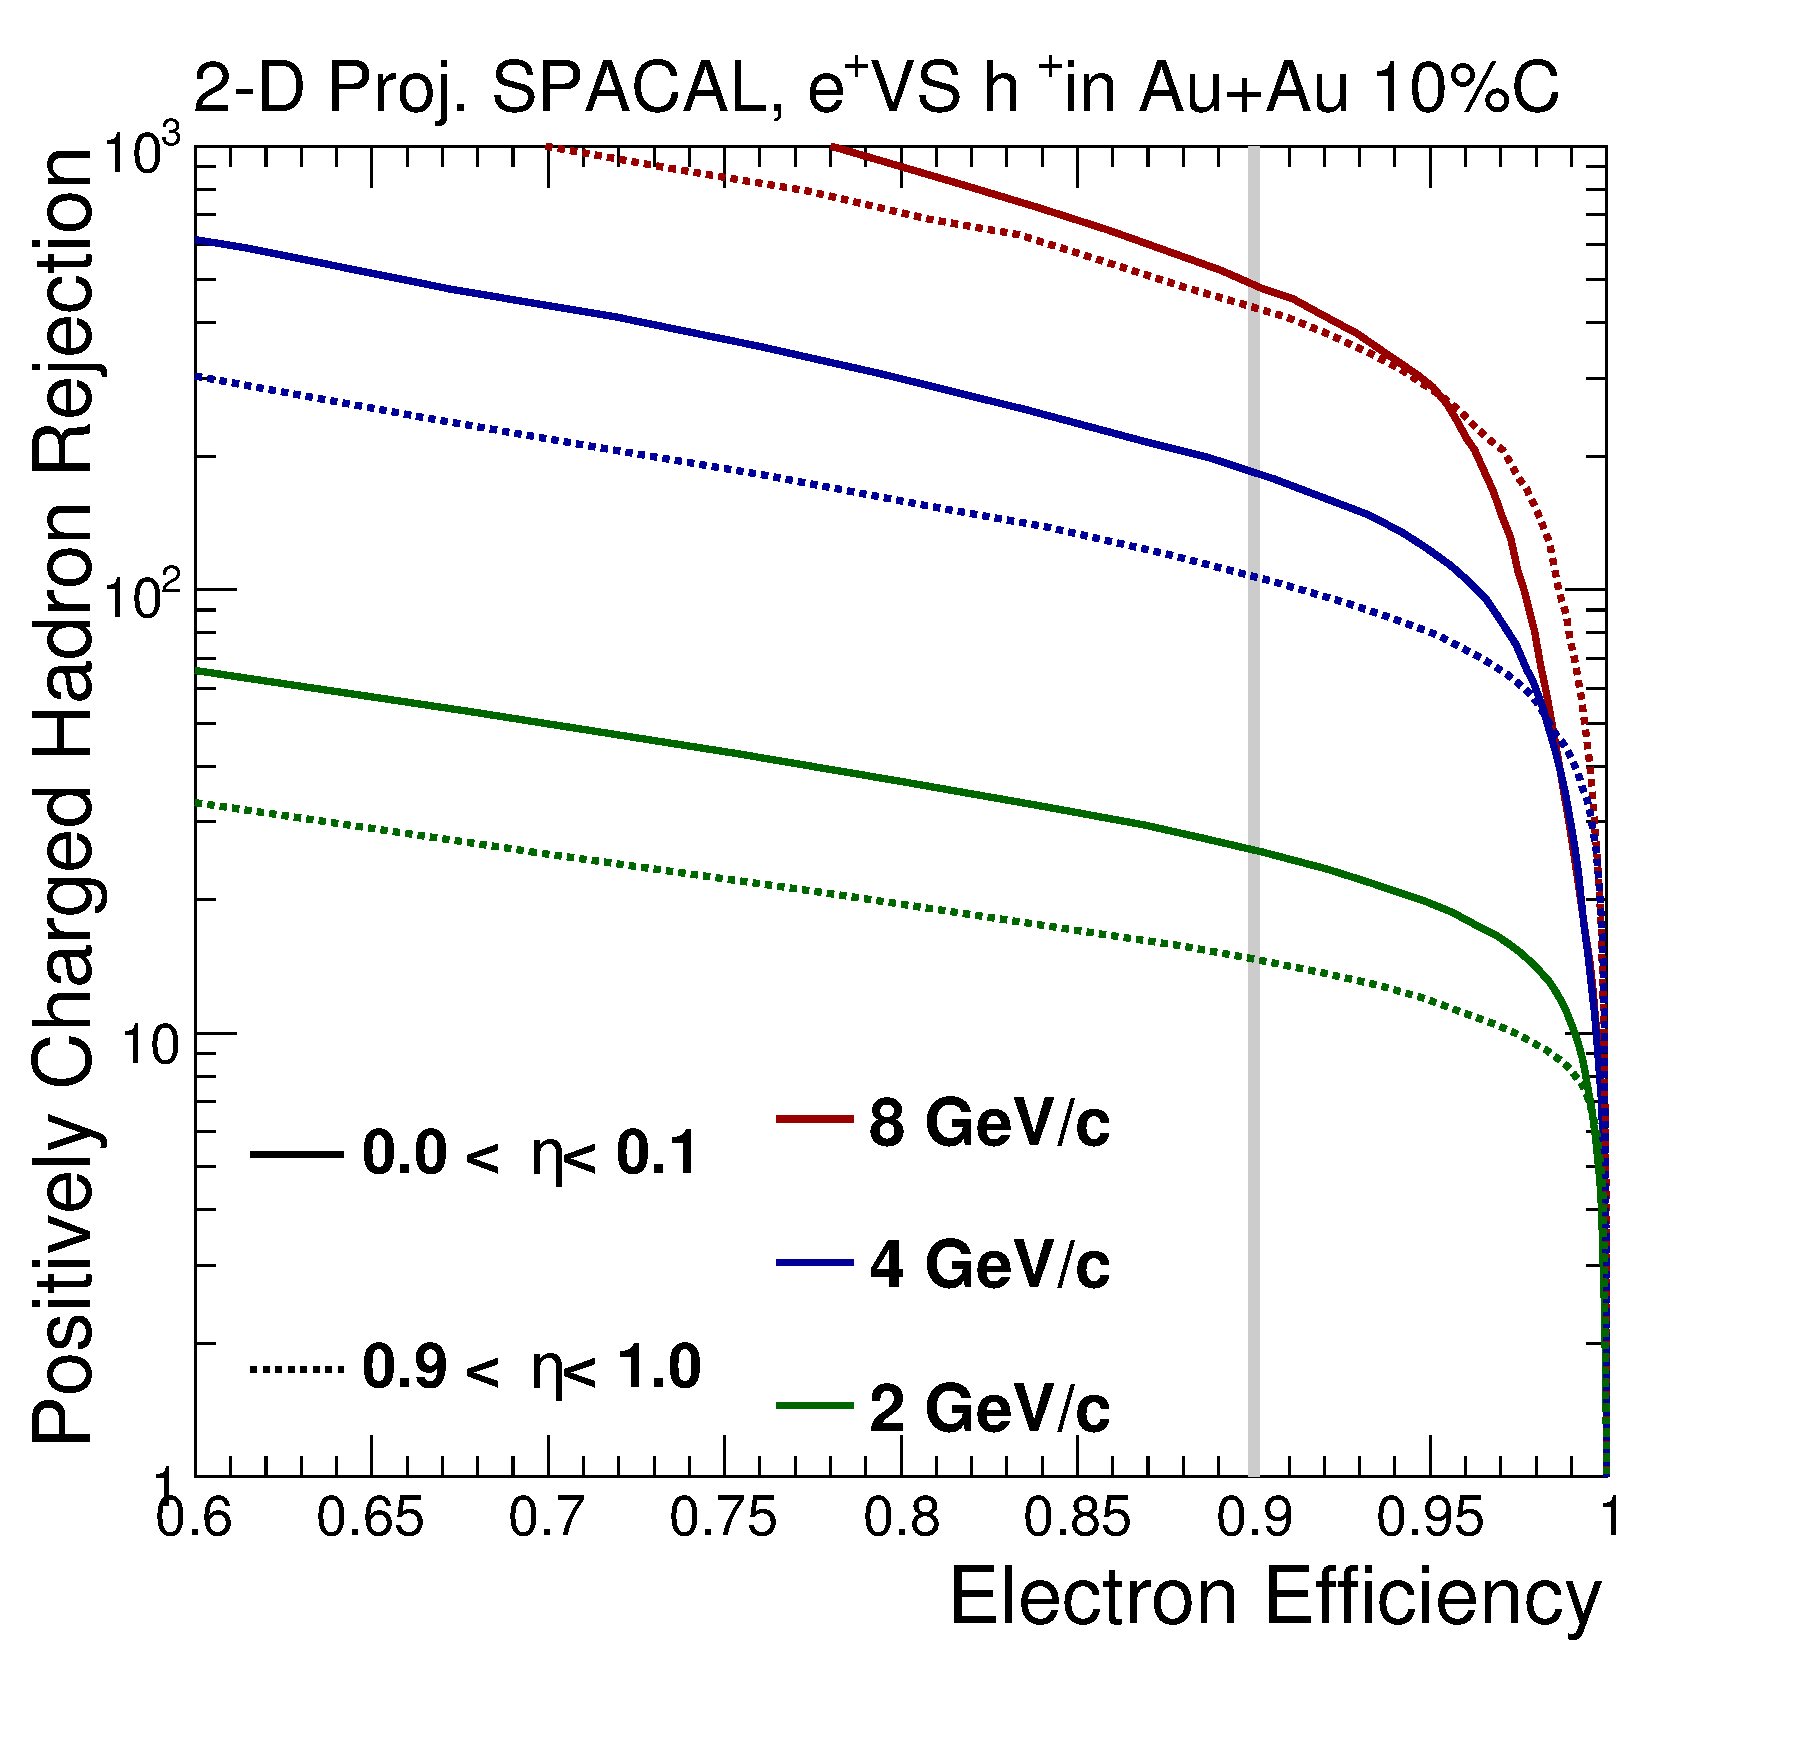
\includegraphics[width=0.4\linewidth]{figs/DrawEcal_Likelihood_Sum_RejectionCurve_AuAuSummaryPos}
  \caption{For a $2\times2$ ganged EMCal (with inner HCal present)
    inclusive charged hadron rejection is plotted on the left (right)
    as function of electron ID efficiency, for negatively (positively)
    charged tracks of three choices of momentum and for middle and
    edge rapidity in 10\% most central Au+Au events.}
  \label{fig:eid_auau}
\end{figure}

\begin{figure}[hbt]
  \centering
  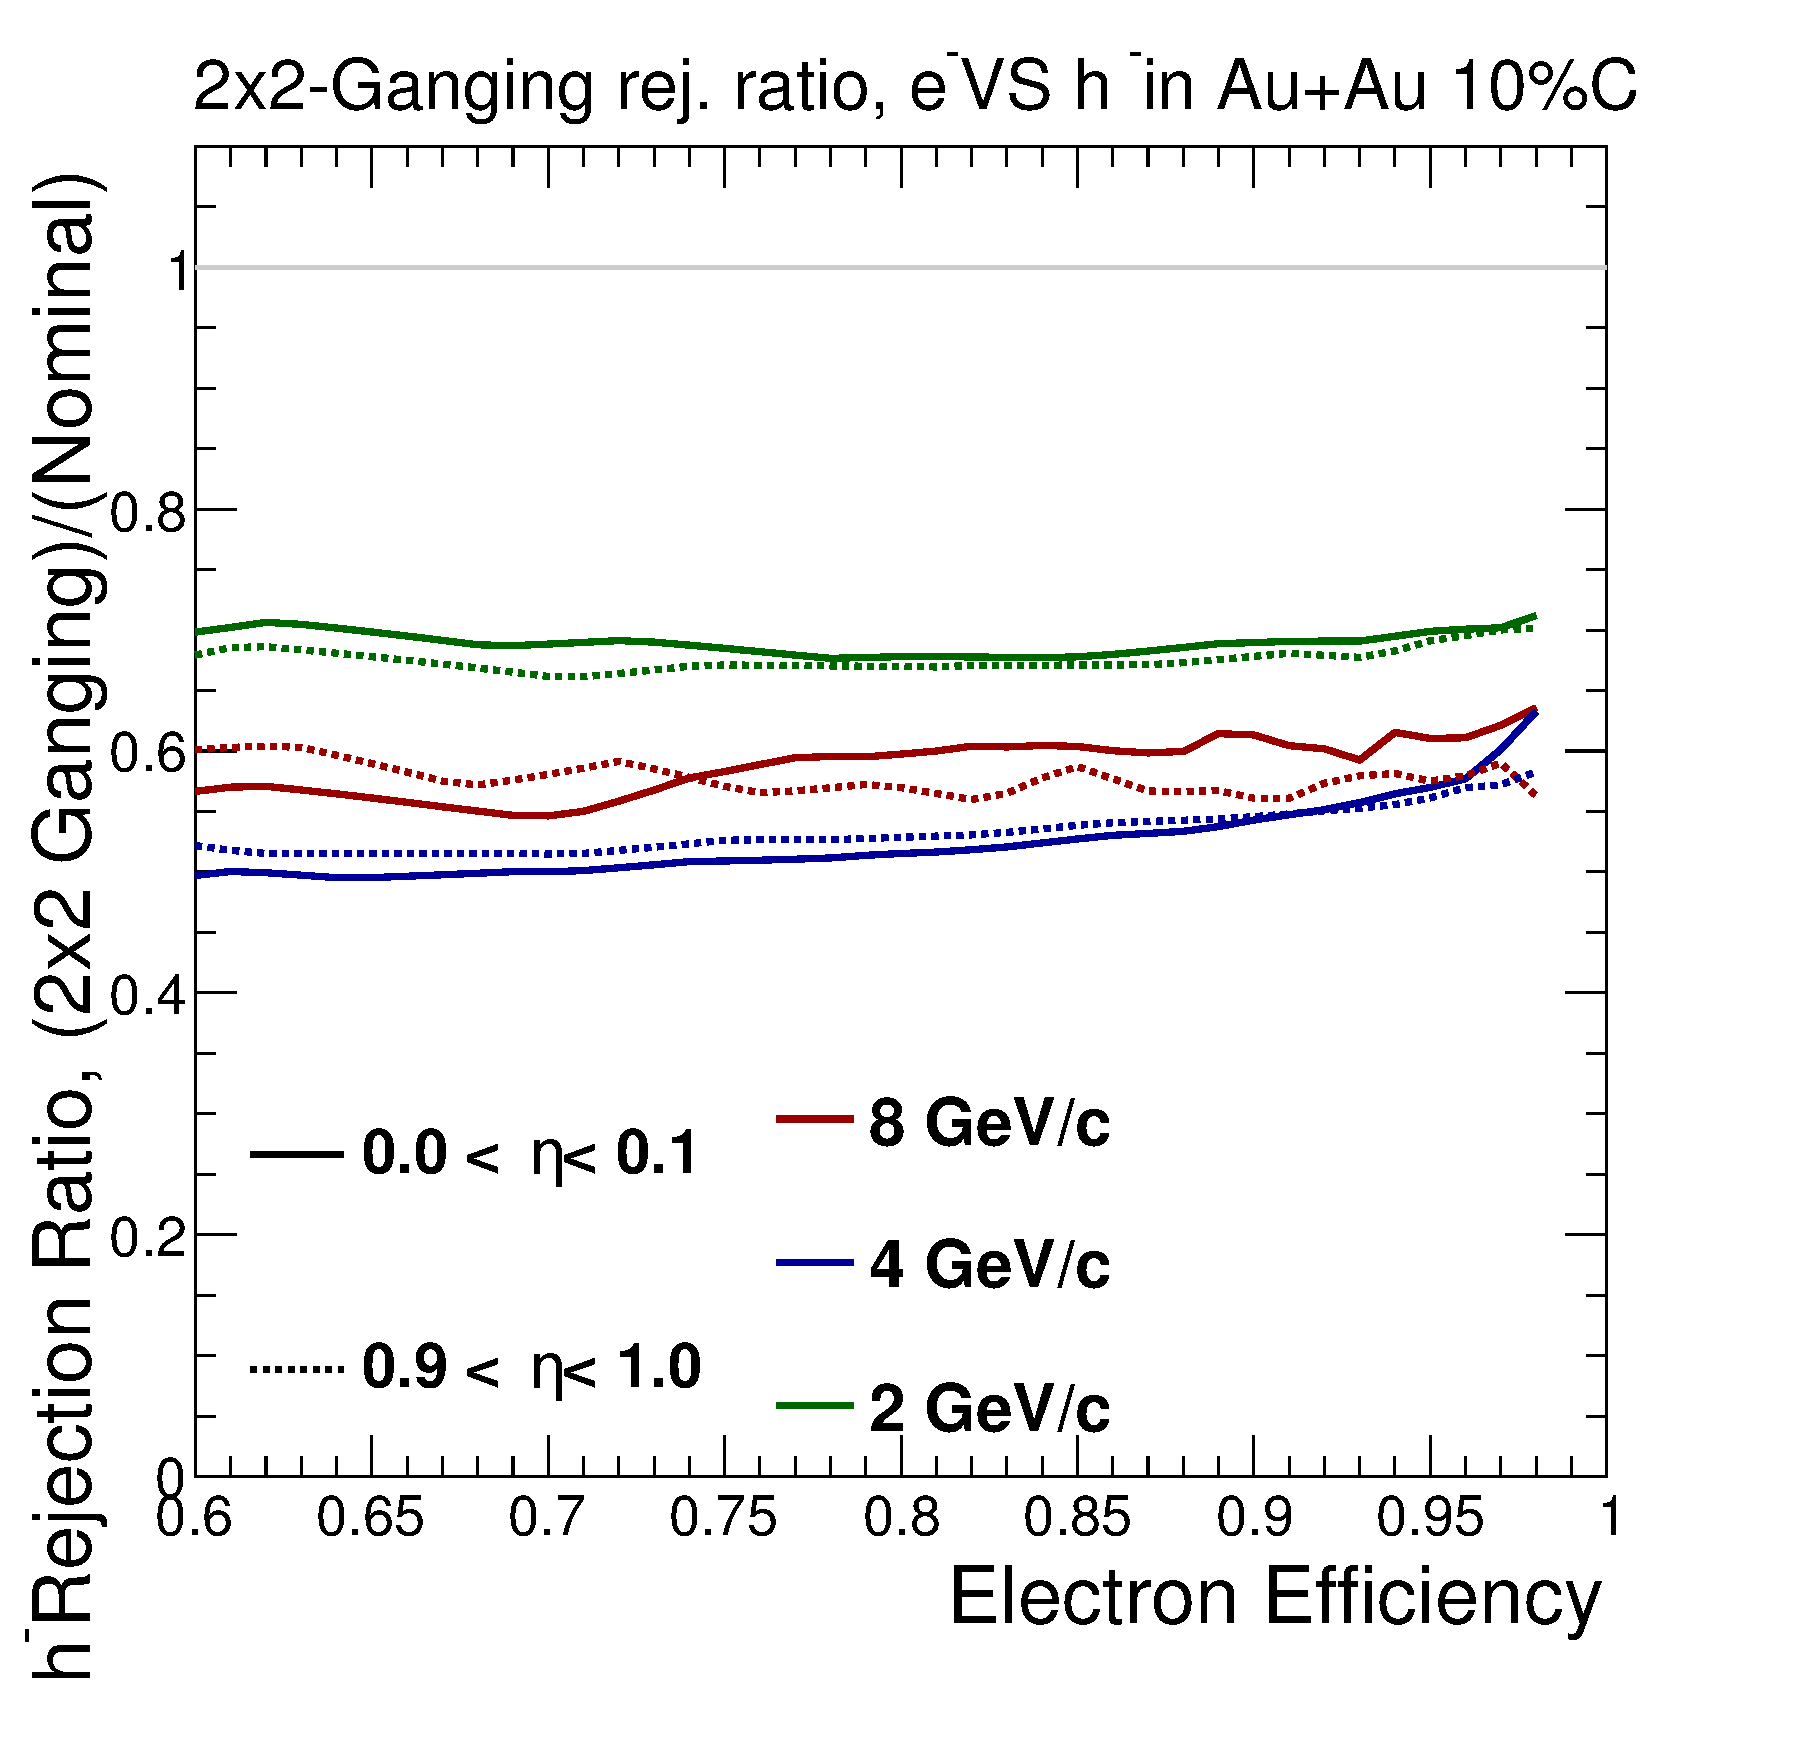
\includegraphics[width=0.6\linewidth]{figs/DrawEcal_Likelihood_Sum_RejectionCurve_AuAuSummary_Compare}
  \caption{ Ratios of inclusive charged hadron rejection of $2\times2$
    ganged EMCal to the reference design, as functions of electron ID
    efficiency. This is evaluated for negatively charged tracks of
    three choices of momentum and for middle and edge rapidity in 10\%
    most central Au+Au events.}
\label{fig:eid_ratios_auau}
\end{figure}

\begin{figure}[hbt]
  \centering
  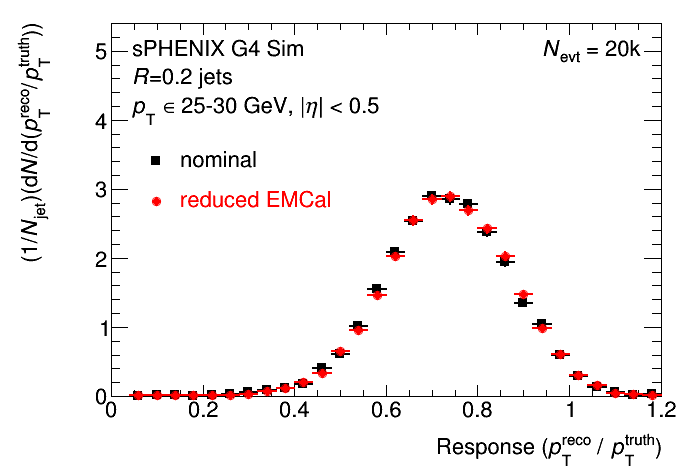
\includegraphics[width=0.4\linewidth]{figs/jet_response_reduced_emcal_eta_0} \\
  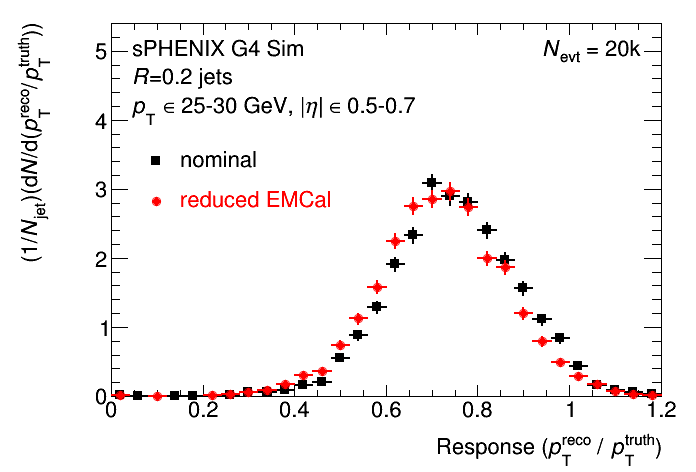
\includegraphics[width=0.4\linewidth]{figs/jet_response_reduced_emcal_eta_05} \\
  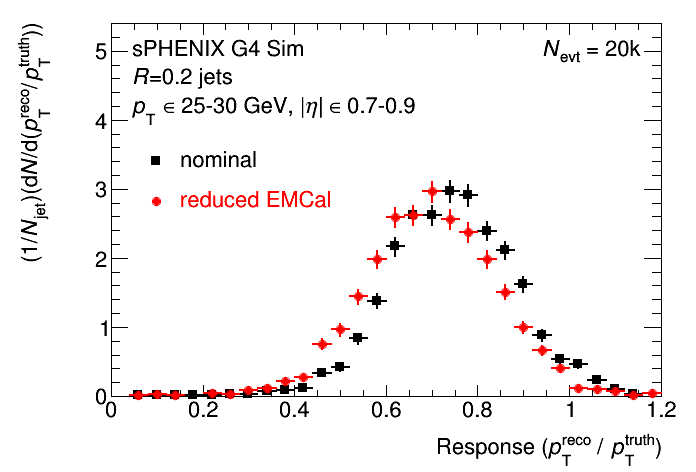
\includegraphics[width=0.4\linewidth]{figs/jet_response_reduced_emcal_eta_07}
  \caption{The effect on the jet response on reducing the EMCal to an acceptance within |eta|<0.6 was also examined with full \geant simulations.}
  \label{fig:jet_response_reduced_emcal}
\end{figure}

